% !TeX root = main.tex

\section{Validation des données et interface utilisateur}
\label{sec:fiabilisation}

Ce chapitre présente la phase de validation des données extraites automatiquement et l'interface développée pour les opérateurs du cabinet. Il détaille le fonctionnement de l'application Streamlit, la gestion de l'état en mémoire, les règles de contrôle de cohérence, ainsi que les outils de recherche et de géolocalisation nécessaires avant l'exportation vers Géofoncier.


\subsection{Principes et fonctionnement de l'application Streamlit}

Le traitement des archives présenté au chapitre précédent produit des résultats sur la grande majorité des documents. Cependant, il est impossible de s'en remettre entièrement à ce type de détection pour verser des données sur un portail national à but juridique. Les informations extraites alimentent le Référentiel Foncier Unifié (RFU) de Géofoncier. Une erreur sur le nom d'une commune, sur la section cadastrale ou sur le numéro d'un dossier génère une pastille pouvant être mal localisée, voire une fiche indexée sous le mauvais acte foncier. Compte tenu de la valeur juridique de ces documents, ce type d'erreur n'est pas tolérable.

L'OCR produit parfois des chaînes de caractères incorrectes car la source même de la donnée peut être dégradée, et le modèle VLM retourne la mention \texttt{INCERTAIN} lorsqu'il ne parvient pas à trouver une réponse. Dans tous ces cas de figure, seule une vérification humaine valide la donnée. L'interface de validation assiste l'opérateur en lui présentant le document et les données extraites côte à côte, en lui signalant les champs soumis à un doute, et en lui fournissant des outils de recherche dans les répertoires existants. Une fois un dossier confirmé par l'opérateur, le fichier CSV correspondant est mis à jour et les données peuvent être transmises à l'API Géofoncier.

L'application est développée en Python avec le framework Streamlit, qui permet de créer des applications web sans écrire de code HTML. Elle s'exécute localement sur la machine du cabinet, accessible depuis n'importe quel navigateur web du réseau local sur le port 8501. Les données restent ainsi confinées au réseau du cabinet, sans transiter par des serveurs externes.

Pour bien comprendre la conception de l'application, il faut prendre en compte le fonctionnement de Streamlit. À chaque fois que l'utilisateur interagit avec l'application (en cliquant sur un bouton ou en modifiant une case), le script Python est intégralement réexécuté du début à la fin. Ce procédé réinitialise la page et effacerait les corrections saisies avant qu'elles ne soient sauvegardées. Pour éviter ce problème, l'application conserve les modifications en cours dans une mémoire temporaire gérée par la session. Les données modifiées y sont stockées et restent affichées à l'écran tout au long de la relecture du document. La sauvegarde définitive n'intervient que lorsque l'opérateur clique sur le bouton de validation.

La gestion de cette mémoire de session s'organise autour de plusieurs variables conservées d'une exécution à l'autre :
\begin{itemize}
  \item \textbf{L'index du document} : conserve la position du document actuellement affiché dans le lot de travail sélectionné.
  \item \textbf{Les valeurs du document} : mémorisent l'ensemble des données des champs d'indexation (commune, section, date, géomètre, parcelles) et mettent à jour les champs en temps réel dès qu'une modification est saisie.
  \item \textbf{Les indicateurs de confiance} : conservent les scores d'exactitude et les alertes associées à chaque champ pour adapter la couleur des badges visuels.
  \item \textbf{L'historique local des corrections} : enregistre les paires de valeurs corrigées pour proposer des suggestions automatiques si la même erreur survient sur d'autres pièces du même lot.
\end{itemize}

Grâce à cette architecture, l'opérateur peut naviguer dans le document, ajuster le zoom de l'image scannée et modifier plusieurs champs sans subir de réinitialisation impromptue des saisies.





\subsection{Structure de l'interface et formulaire de correction}

L'écran principal de l'application (Figure~\ref{fig:interface_haut}) s'ouvre sur un en-tête intitulé \enquote{Validation des archives cadastrales}. Dans la barre supérieure, l'opérateur choisit son fichier de travail dans le menu déroulant \enquote{Fichier de travail}, consulte l'identifiant du document chargé (par exemple \texttt{07110\_000\_160} pour la commune de Joyeuse), ainsi que le compteur de progression du lot en cours (\texttt{0 / 1 documents validés}).

L'espace de travail est structuré en deux colonnes principales :
\begin{itemize}
  \item La colonne de gauche, intitulée \enquote{SAISIE \& CORRECTION}, regroupe l'ensemble des champs d'indexation sous la forme d'un formulaire interactif organisé par groupes (\textit{Localisation}, \textit{Références \& Acte}, \textit{Intervenants}, et \textit{Parcelles}).
  \item La colonne de droite, intitulée \enquote{APERÇU DU DOCUMENT (ZOOM INTERACTIF)}, affiche l'image scannée du plan cadastral.
\end{itemize}

\begin{figure}[H]
  \centering
  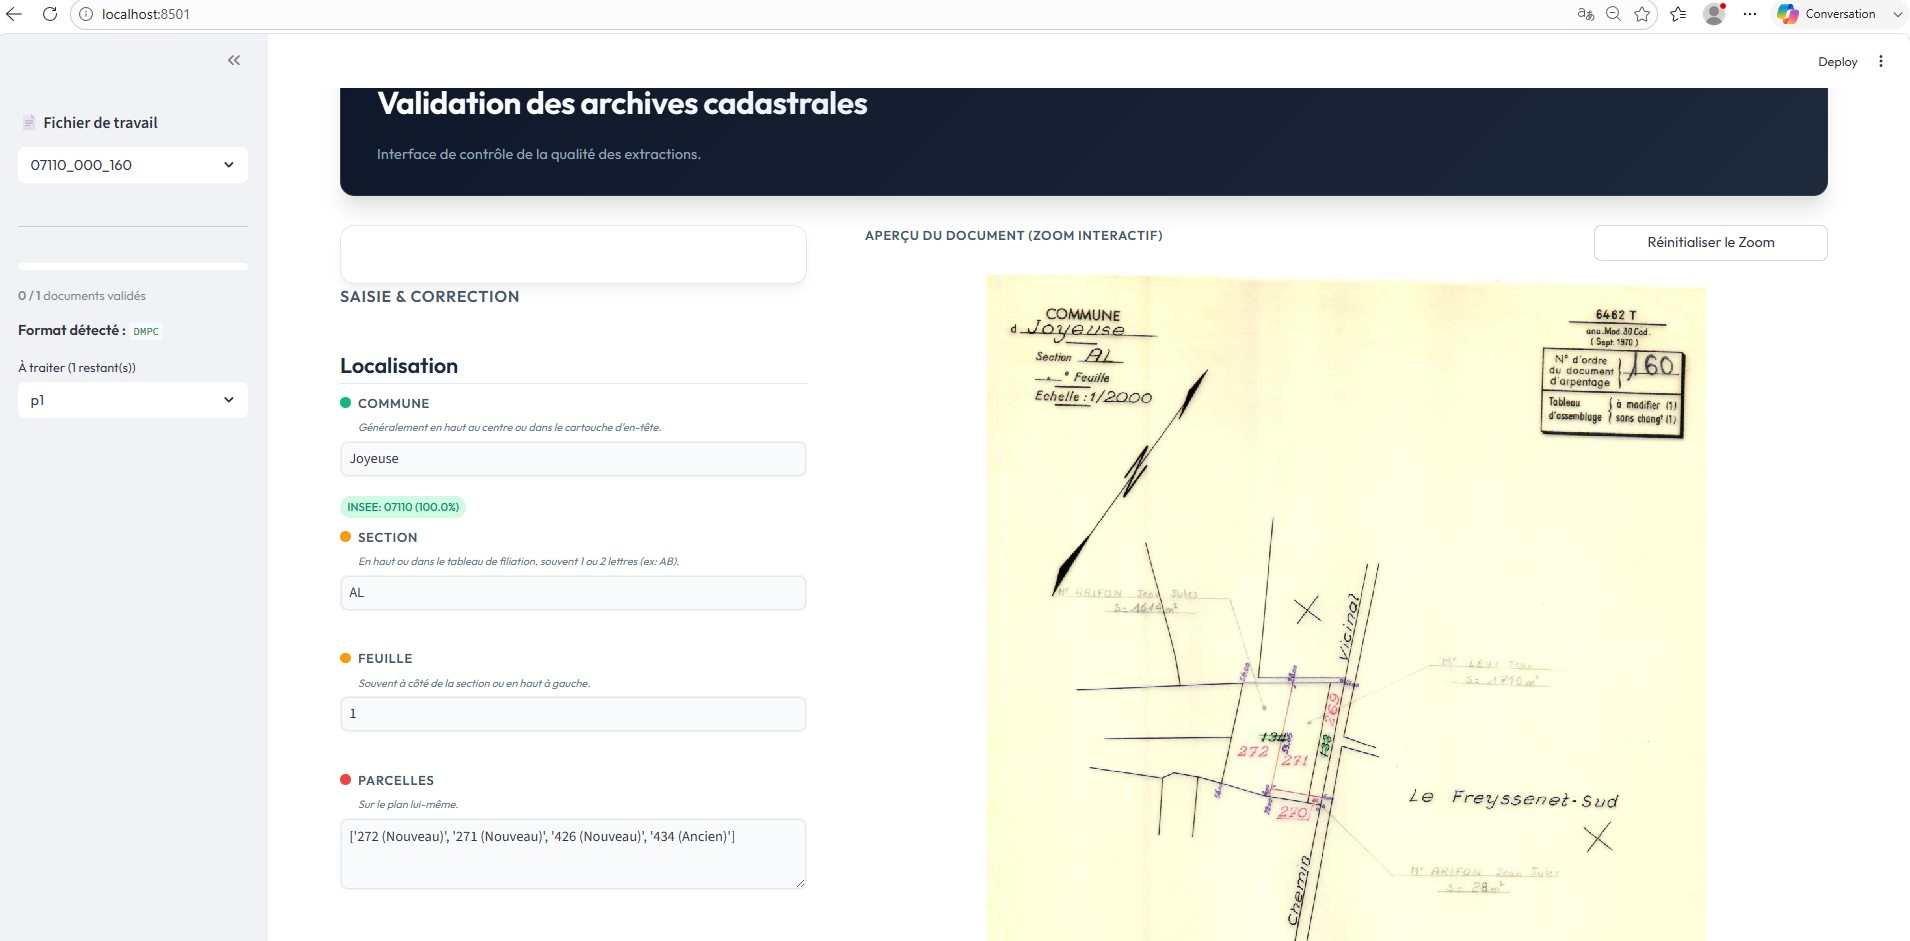
\includegraphics[width=1\textwidth]{img/interface_haut.jpg}
  \caption{Partie supérieure de l'interface de validation, montrant l'en-tête, le sélecteur de fichier, l'identifiant du document \texttt{07110\_000\_160} et la disposition en deux colonnes.}
  \label{fig:interface_haut}
\end{figure}

La colonne de gauche regroupe les champs à vérifier sous la forme d'une liste d'éléments organisés en plusieurs groupes (\textit{Localisation}, \textit{Références \& acte}, \textit{Intervenants}, et \textit{Parcelles}). Pour chaque champ, l'interface affiche la valeur extraite et une couleur indiquant le niveau de confiance.

Comme l'illustre l'extrait de la Figure~\ref{fig:zoom_commune}, le champ \texttt{COMMUNE} affiche la valeur extraite \texttt{Joyeuse} accompagnée du code \texttt{INSEE: 07110 (100.0\%)}, qui confirme la correspondance avec le référentiel des communes.

\begin{figure}[H]
  \centering
  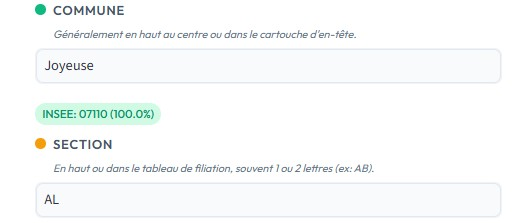
\includegraphics[width=0.65\textwidth]{img/zoom_commune.jpg}
  \caption{Extrait du formulaire de correction montrant le champ Commune .}
  \label{fig:zoom_commune}
\end{figure}

Dans la colonne de droite, un outil de navigation permet de zoomer sur le document et de se déplacer dans l'image pour examiner les champs. Un bouton \enquote{Réinitialiser le Zoom} placé au-dessus de l'image permet de réinitialiser l'affichage à tout moment.


Quand l'opérateur modifie une valeur dans le document, l'application applique une normalisation automatique : mise en majuscules de la section, formatage de la date en \texttt{JJ/MM/AAAA}, nettoyage des séparateurs de parcelles et résolution du code INSEE via la base de données des communes.

L'application mémorise également les corrections apportées par l'opérateur. Quand il corrige un champ (commune, géomètre, section, nature de l'acte...), la correspondance entre la valeur extraite et la valeur corrigée est sauvegardée. Sur les documents suivants du même fonds, si l'application retrouve la même valeur erronée, elle la remplace automatiquement, et affiche un badge \enquote{Auto-corrigé} à côté du champ pour le signaler. Concrètement, une erreur répétée, comme un nom de commune systématiquement mal lu, n'a besoin d'être corrigée qu'une seule fois pour tout une série de scans.


\subsection{Recherche dans les répertoires et géolocalisation}

Une fois les champs validés, l'interface bascule sur un second écran organisé en trois étapes.

Pour retrouver le numéro de dossier original dans les répertoires du cabinet, l'opérateur utilise d'abord le formulaire de recherche (Figure~\ref{fig:etape1_recherche}). Ce formulaire comporte quatre champs : commune, section cadastrale, numéro de parcelle et année. Les valeurs pré-remplies proviennent de l'étape de détection automatique (chapitre~\ref{sec:architecture}), mais l'opérateur peut les ajuster en cas d'erreur. Un clic sur le bouton \enquote{Rechercher dans le répertoire} interroge le fichier du géomètre concerné, en s'appuyant sur les identifiants cadastraux ou sur les noms de propriétaires. 

\begin{figure}[H]
  \centering
  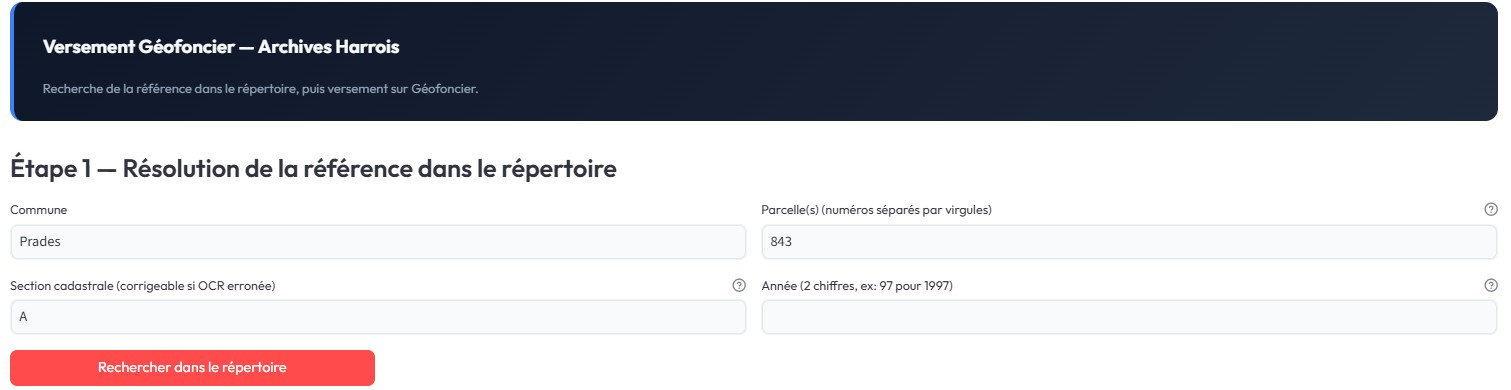
\includegraphics[width=0.85\textwidth]{img/Etape 1_recherche_reference.jpg}
  \caption{Étape 1 -- Formulaire de recherche et de résolution de la référence dans le répertoire.}
  \label{fig:etape1_recherche}
\end{figure}

Lorsque la recherche donne une correspondance unique, celle-ci est directement affichée et validée dans un encadré vert. En revanche, si plusieurs dossiers correspondent aux critères saisis, l'application présente un tableau de choix permettant à l'opérateur de sélectionner la référence exacte avant de poursuivre.

\begin{figure}[H]
  \centering
  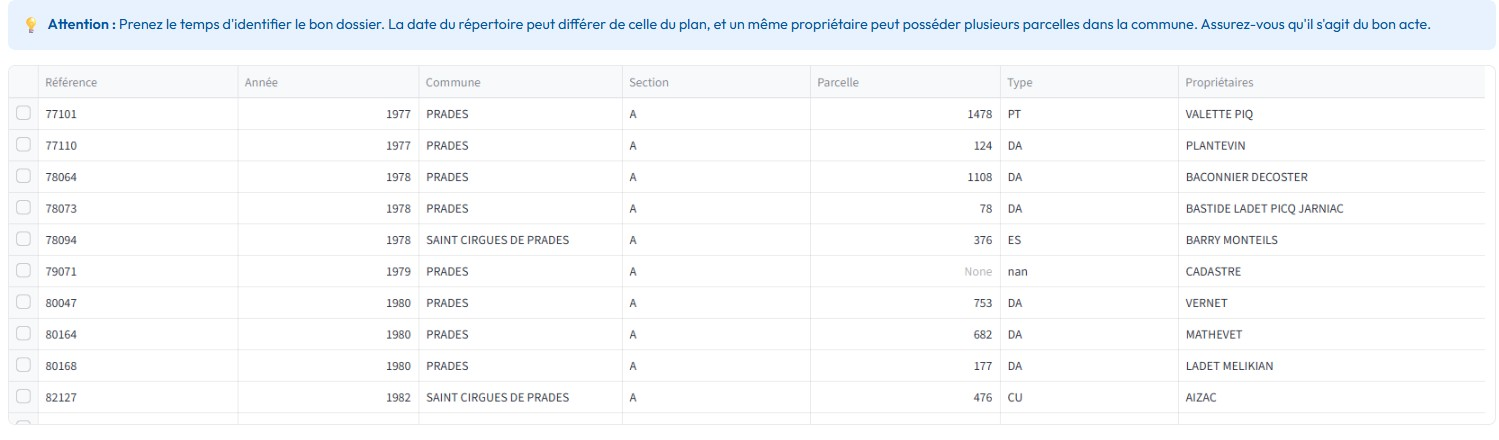
\includegraphics[width=0.85\textwidth]{img/etape_1_liste_possibilites.jpg}
  \caption{Étape 1 -- Tableau de sélection parmi plusieurs dossiers candidats en cas d'ambiguïté.}
  \label{fig:etape1_candidats}
\end{figure}

Comme illustré Figure~\ref{fig:etape1_candidats}, l'opérateur doit trancher manuellement en s'appuyant sur les informations disponibles dans le tableau. L'année de l'acte et les noms des propriétaires sont généralement les éléments les plus fiables pour identifier le bon dossier, notamment lorsque plusieurs opérations portent sur la même parcelle.

Une fois la référence du dossier confirmée, l'interface passe automatiquement à la phase de localisation cartographique.

L'étape suivante s'appuie sur une carte interactive intégrée via la bibliothèque Folium. Lors du chargement de la commune validée, l'application interroge le service WFS de la DGFiP ou de l'IGN pour récupérer l'emprise vectorielle de la parcelle cadastrale ou du centroïde communal. La carte centre automatiquement l'affichage sur la zone d'intervention et superpose deux couches d'information : le réseau des parcelles cadastrales actuelles et la couche des pastilles d'opérations déjà versées sur le portail GéofoncierEXPERT.

L'opérateur peut déplacer le marqueur d'un simple clic sur le fond de carte pour affiner la localisation de la pastille en cas d'imprécision sur le centroïde calculé. Si la parcelle d'origine a fait l'objet d'une division récente, le module de filiation parcellaire (décrit au chapitre~\ref{sec:analyse_metier}) affiche l'historique des parcelles filles en surbrillance, ce qui permet à l'opérateur de valider le positionnement géographique même si le découpage cadastral actuel ne correspond plus exactement à l'extrait du plan ancien.

Cette deuxième étape ouvre la carte interactive (Figure~\ref{fig:etape2_carte}) superposant le fond cadastral IGN et les pastilles Géofoncier déjà existantes. Un bandeau d'avertissement invite l'opérateur à s'assurer qu'aucun doublon n'a été déposé auparavant. Si la parcelle d'origine a fait l'objet de divisions depuis la création du plan, l'application identifie automatiquement la filiation foncière : un message vert indique les numéros actuels issus de la division (par exemple, la parcelle A-840 devenue A-1618, 1649, 1650 et 1967) et affiche leurs contours en violet sur la carte. L'opérateur peut aussi cliquer sur le bouton \enquote{Comparer avec le plan d'époque} pour ajuster visuellement le calage. Une fois l’emplacement validé ou ajusté sur la carte, la localisation est verrouillée pour l'export.

\begin{figure}[H]
  \centering
  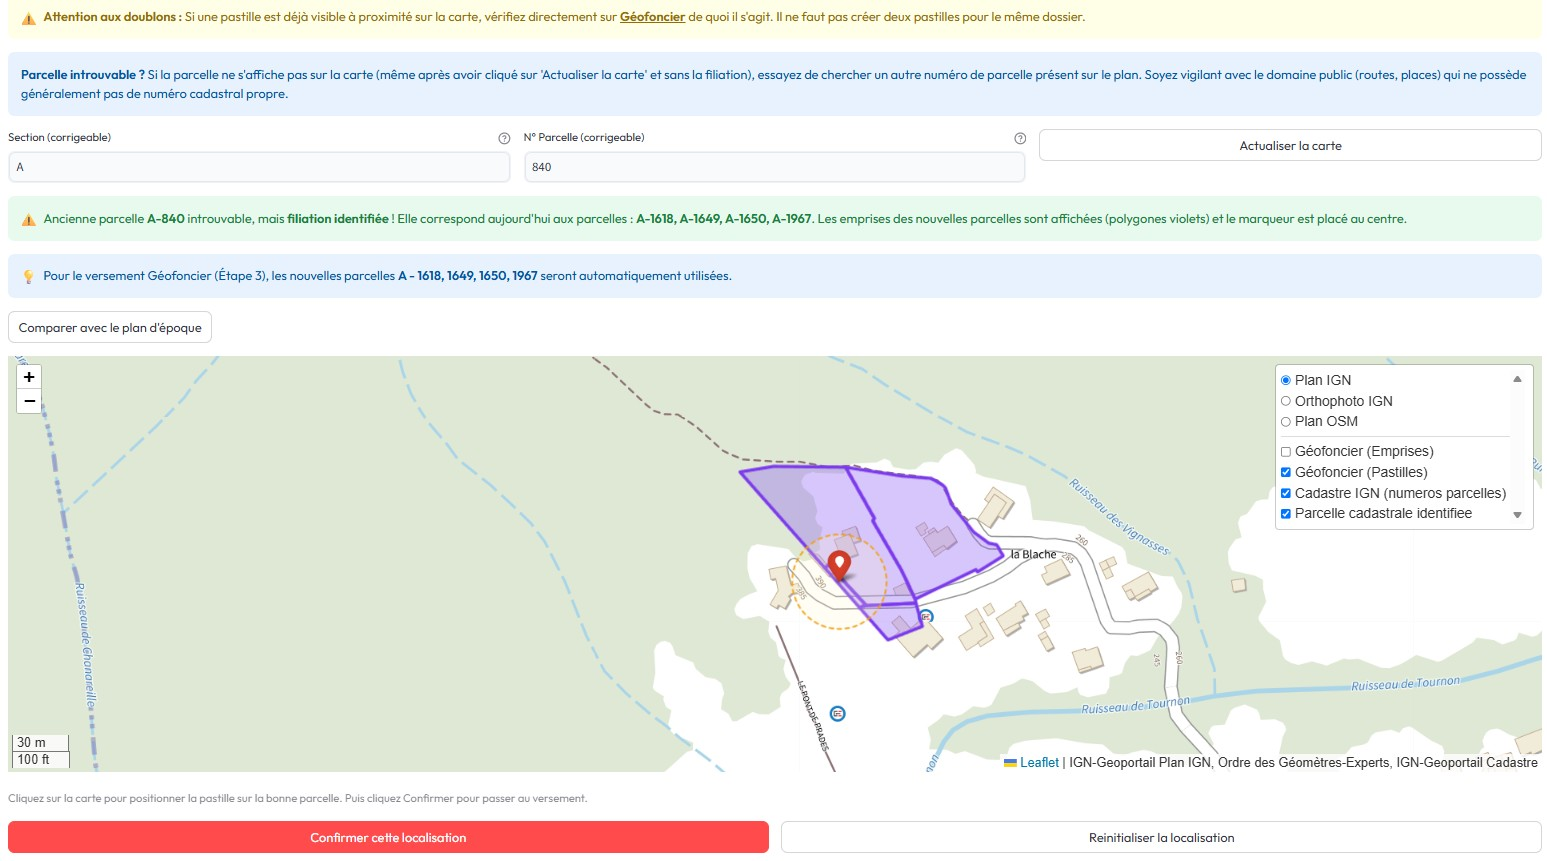
\includegraphics[width=0.95\textwidth]{img/Etape_2_localisation_cartographie.jpg}
  \caption{Étape 2 -- Carte interactive avec fond cadastral IGN, gestion des filiations de parcelles et contrôle des doublons Géofoncier.}
  \label{fig:etape2_carte}
\end{figure}

Après cette validation, l'application oriente l'utilisateur vers la phase finale du traitement.


\subsection{Exportation et versement sur Géofoncier}

La dernière étape regroupe l'ensemble des informations collectées pour l'envoi vers Géofoncier. Le récapitulatif est divisé en deux sections : la première rassemble les données du cabinet (cabinet créateur, détenteur, géomètre et référence interne du dossier), tandis que la seconde récapitule les éléments cadastraux (code INSEE, commune, section, parcelles retenues et nature de l'acte). Le type d'opération est rempli automatiquement. L'opérateur précise la date, choisit le statut dans la liste déroulante et vérifie les éventuels messages d'avertissement. Enfin, l'activation du bouton \enquote{Créer le dossier sur Géofoncier} déclenche l'envoi vers l'API REST pour inscrire le dossier sur la plateforme.

\begin{figure}[H]
  \centering
  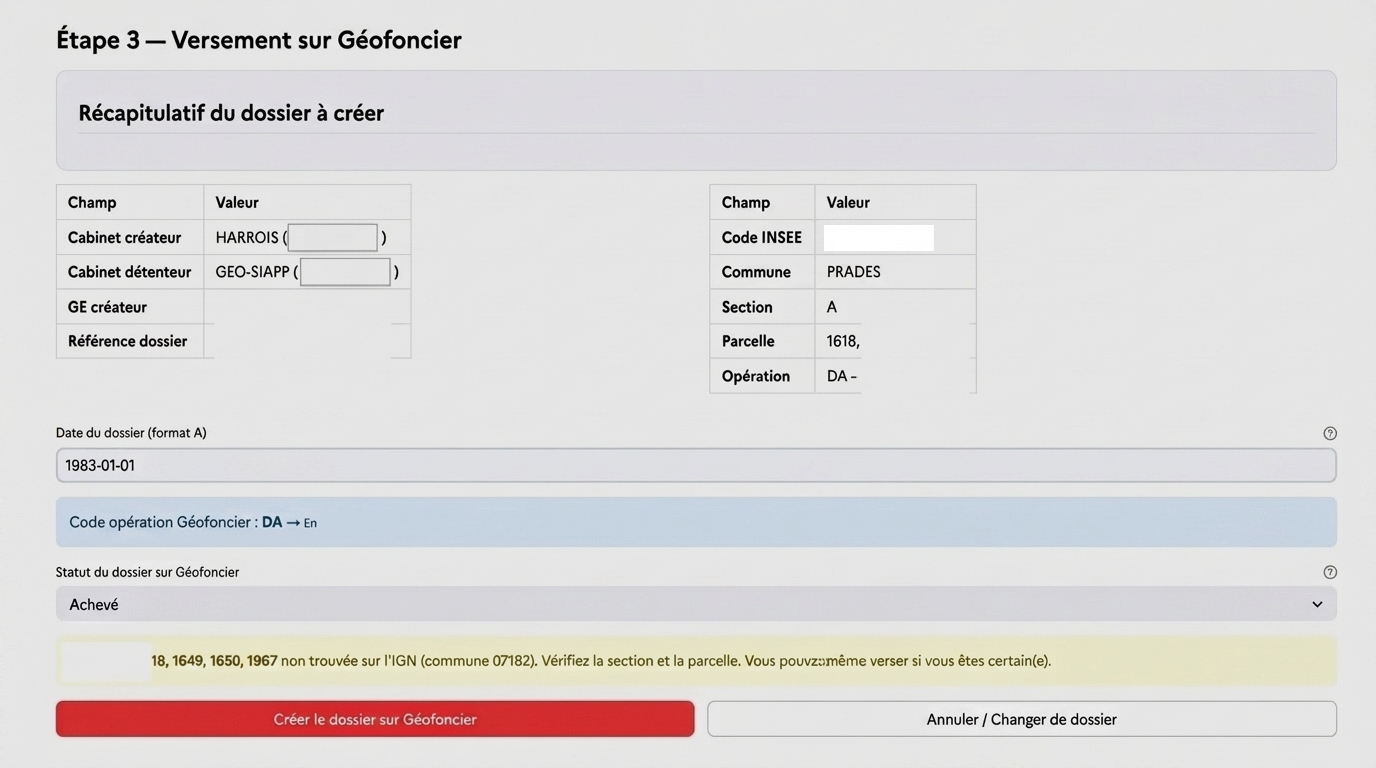
\includegraphics[width=0.90\textwidth]{img/Etape3_Versement_geofoncier.jpg}
  \caption{Étape 3 -- Formulaire de versement sur Géofoncier avec récapitulatif des données du cabinet et des éléments cadastraux.}
  \label{fig:etape3_versement}
\end{figure}



\subsection{Numérisation des répertoires anciens}

La recherche dans les répertoires présentée à la section précédente repose sur des fichiers Excel qui listent l'ensemble des dossiers archivés par chaque géomètre. Ces fichiers n'existaient pas sous forme numérique pour certains, les répertoires du Géomètre A et du Géomètre B n'étaient disponibles que sous forme de registres papier manuscrits, numérisés en PDF. Deux programmes d'extraction indépendants ont été développés dans le cadre de ce PFE pour produire ces bases de données, chacun adapté à la mise en page et à la nature des écritures du géomètre concerné. Les deux suivent la même structure en deux temps : une phase d'extraction automatique, suivie d'une interface de validation. Chacun est lancé par un fichier \texttt{.bat} qui installe les dépendances manquantes, exécute l'extraction, puis ouvre l'interface dans le navigateur web.

Le registre du Géomètre A (Figure~\ref{fig:geom_a_liste}) se présente sous la forme d'un tableau à double colonne : la colonne de gauche liste les anciens propriétaires, la colonne de droite les nouveaux. Les années sont imprimées en rouge et encadrent les blocs de dossiers. Les numéros de dossiers, portés dans la marge gauche, servent d'ancres pour délimiter chaque entrée. Le script \texttt{extract\_geometre\_A.py} traite les PDF page par page à haute résolution (environ 288 DPI). EasyOCR retourne les blocs de texte avec leurs coordonnées. Une analyse de l'image localise ensuite la ligne verticale qui sépare les deux colonnes de propriétaires. Les blocs dont le fond est détecté comme rouge en espace HSV sont extraits comme marqueurs d'année. Une correction rectifie les confusions dues au soulignement rouge qui coupe certains chiffres (un \texttt{1913} lu par l'OCR peut être corrigé en \texttt{1973} si l'année sort de la plage attendue). Les numéros de dossiers dans la marge gauche servent d'ancres : chaque bloc de texte est assigné au dossier dont l'ancre est la plus proche en Y, puis affecté à la colonne \textit{Anciens} ou \textit{Nouveaux} selon sa position par rapport au séparateur. Les communes sont résolues par correspondance (\texttt{rapidfuzz}) contre la liste des communes de l'Ardèche et de la Drôme. Les dossiers extraits sont enregistrés dans un fichier JSON intermédiaire en attendant la validation.

\begin{figure}[H]
  \centering
  \setlength{\fboxsep}{0pt}%
  \setlength{\fboxrule}{0.6pt}%
  \fbox{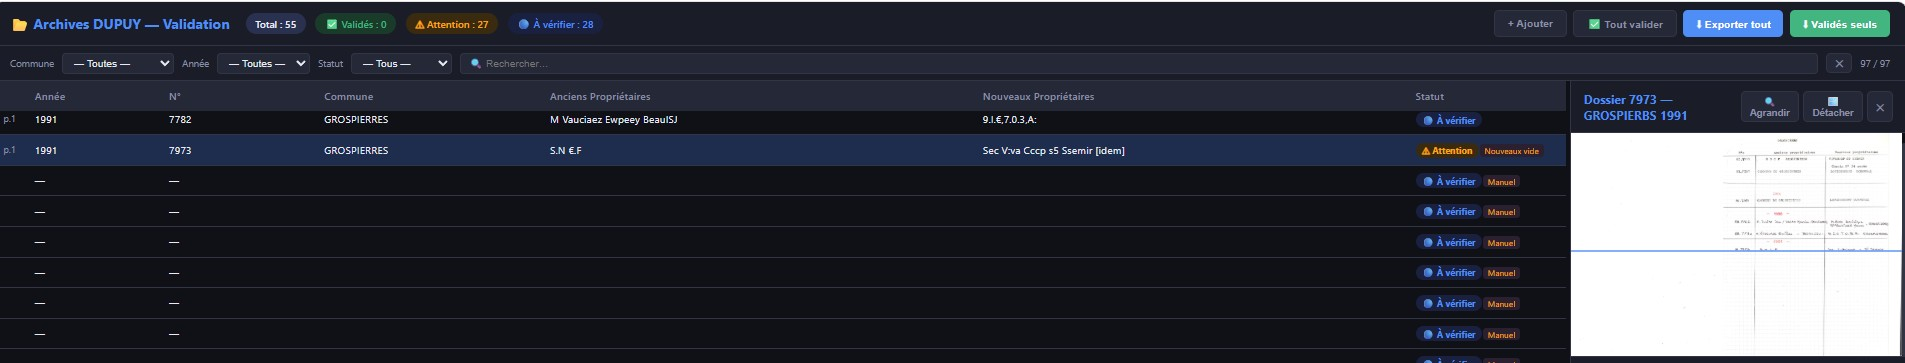
\includegraphics[width=0.95\linewidth]{img/5.5_reprtoire_A_liste.jpg}}
  \caption{Interface de validation du répertoire du Géomètre A (port 5050) -- Vue synthétique et liste des dossiers extraits.}
  \label{fig:geom_a_liste}
\end{figure}

\clearpage

\begin{wrapfigure}{r}{0.46\textwidth}
  \vspace{-1.2em}
  \centering
  \setlength{\fboxsep}{0pt}%
  \setlength{\fboxrule}{0.6pt}%
  \fbox{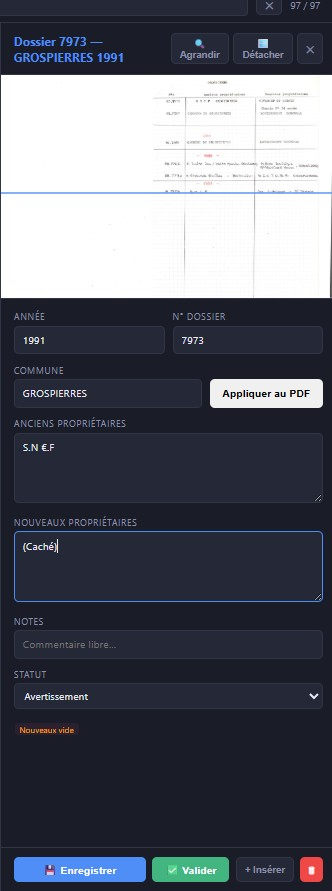
\includegraphics[width=\linewidth]{img/5.5_reprtoire_A_infos.jpg}}
  \caption{Interface du Géomètre A (port 5050) -- Fiche détaillée et édition des champs.}
  \label{fig:geom_a_infos}
  \vspace{-1em}
\end{wrapfigure}

L'interface de validation est un serveur local accessible sur \texttt{http://localhost:5050}. Elle s'articule autour de deux vues principales. La première vue (Figure~\ref{fig:geom_a_liste}) présente la liste des dossiers extraits sous la forme d'un tableau synthétique, permettant à l'opérateur de parcourir rapidement l'ensemble des affaires répertoriées.

Lorsqu'un dossier est sélectionné dans le tableau, l'interface affiche la fiche détaillée (Figure~\ref{fig:geom_a_infos}) regroupant l'ensemble des champs d'indexation (commune, année, référence du dossier, anciens et nouveaux propriétaires). L'opérateur peut y consulter le scan de la page originale, réexécuter l'OCR sur une zone spécifique ou corriger directement les valeurs extraites.

À la validation, les corrections sont fusionnées dans le fichier Excel maître (\texttt{Repertoire\_}\linebreak[0]\texttt{Archives\_}\linebreak[0]\texttt{geometre\_A.xlsx}), en utilisant les clés d'indexation (Commune, Année, N° Dossier) pour éviter tout doublon. Ce fichier est également synchronisé sur le serveur partagé du cabinet. (Les captures grand format sont consultables en Annexe G).

Le traitement du registre du Géomètre A repose sur une logique de découpage par colonnes fixes. Les lignes de séparation imprimées en rouge permettent d'isoler les noms des anciens et des nouveaux propriétaires avec un bon taux de réussite. En cas de doute sur une lettre ou un nom propre, l'interface de validation permet à l'opérateur de visualiser immédiatement le bloc d'image découpé et de rectifier la saisie en quelques secondes.

Le registre du Géomètre B présente des difficultés plus importantes en raison de son écriture manuscrite variée et de l'absence de colonnes imprimées. Pour limiter les erreurs de lecture, le script d'extraction applique un prétraitement d'image adaptatif qui redresse la page, ajuste le contraste et cherche les vallées de texte avant de transmettre l'image au modèle VLM. Malgré ces préconisations, les zones raturées et les écritures cursives inclinées exigent une relecture attentive par l'utilisateur avant l'enregistrement final dans le registre maître.

Le registre du Géomètre B est d'une nature différente : il s'agit d'un livret à double page (un aperçu de ce type de registre est présenté en Figure~\ref{fig:registre_ancien}), où chaque ligne correspond à un dossier, répartie en cinq colonnes (numéro de dossier, date, commune, désignation de l'affaire, donneur d'ordre). L'écriture est manuelle et les colonnes ne sont pas toujours parfaitement alignées, ce qui rend l'OCR seul insuffisant. Le script \texttt{extract\_geometre\_B.py} adopte pour cela une stratégie hybride. Les PDF sont rendus à haute résolution et les doubles pages découpées au milieu. Un redressement automatique corrige les légers défauts d'angle liés à la numérisation du livret. EasyOCR localise ensuite les boîtes de texte et les regroupe par ligne selon leur proximité verticale, et les en-têtes de colonnes sont exclus automatiquement. Chaque ligne est découpée en image, sur laquelle des repères verticaux sont tracés à des positions connues car régulières pour matérialiser les séparations entre colonnes. Cette image annotée est envoyée au modèle IA MiniCPM-V (exécuté localement via Ollama) avec un prompt qui lui demande de lire chaque colonne et de retourner un JSON avec les clés \texttt{N\_Dossier}, \texttt{Date}, \texttt{Commune}, \texttt{Affaire} et \texttt{Client}. Les réponses sont ensuite nettoyées et validées : format de date, résolution de la commune par correspondance contre les communes de l'Ardèche. Un filtre anti-hallucination vide la case commune si aucune correspondance locale n'est trouvée.

L'interface de validation est la même que celle du Géomètre A, accessible sur le port local \texttt{5051}. Elle s'adapte aux informations propres au registre du Géomètre B (numéro de dossier, date, commune, désignation de l'affaire et client). À la validation, les données corrigées sont enregistrées dans un fichier Excel maître distinct (\texttt{Repertoire\_Archives\_}\linebreak[0]\texttt{geometre\_B.xlsx}), en utilisant le triplet (N° Dossier, Date, Commune) comme clé primaire, et le fichier est synchronisé sur le réseau du cabinet.

Cette étape de numérisation préalable des registres permet de construire la base d'indexation indispensable à la recherche d'antériorités. Comme mentionné lors de l'étude des limites au chapitre~\ref{sec:limites_perspectives}, la qualité d'extraction sur ces registres varie selon la régularité des tracés et la présence de lignes de séparation imprimées.


\subsection{Résolution et correction des noms de communes}
\label{subsec:appariement_communes}

Lors de l'extraction des données par les modèles de lecture, le texte transcrit pour les noms de communes contient souvent des erreurs de nature variée : un caractère mal lu, une majuscule différente, une abréviation ou une ligature ancienne. Par exemple, le moteur peut lire \texttt{St-Pierreville} au lieu de \texttt{Saint-Pierreville}, ou \texttt{Chomerac} au lieu de \texttt{Chomérac}. Ces erreurs empêchent une correspondance parfaite avec la liste de référence des communes, ou à l'inverse peuvent faire correspondre une détection à la mauvaise commune.

Pour corriger automatiquement ces écarts, le script s'appuie sur une recherche par correspondance approximative entre la chaîne lue et les noms de communes issus du code officiel de l'INSEE~\citep{insee_cog}. La mesure de similarité utilisée est la \textit{distance de Levenshtein}, qui compte le nombre minimal d'opérations élémentaires (insertion, suppression ou substitution d'un caractère) nécessaires pour transformer une chaîne en une autre~\citep{levenshtein_binary_1966}.

\begin{equation}
  d(a, b) = \min
  \begin{cases}
    d(a_{1..n-1},\, b) + 1 & \text{(suppression)} \\
    d(a,\, b_{1..m-1}) + 1 & \text{(insertion)} \\
    d(a_{1..n-1},\, b_{1..m-1}) + \mathbf{1}_{[a_n \neq b_m]} & \text{(substitution)}
  \end{cases}
\end{equation}

où $a$ est la chaîne extraite, $b$ le nom de commune de référence, $n = |a|$ et $m = |b|$.Le score exprimé sur 100 par la bibliothèque \texttt{rapidfuzz} correspond à un ratio de similarité dérivé de cette distance : $\text{ratio}(a, b) = 100 \times \left(1 - \frac{d(a,b)}{\max(|a|,|b|)}\right)$. Ce score est calculé en quelques microsecondes grâce aux optimisations SIMD de RapidFuzz, ce qui rend la recherche instantanée même sur la liste complète des 40000 communes françaises.

Le script applique plusieurs variantes de correspondance en parallèle pour traiter les cas les plus fréquents :

\begin{itemize}
  \item Correspondance directe normalisée : les deux chaînes sont mises en minuscules, les accents supprimés et les tirets remplacés par des espaces avant la comparaison. Cela résout les différences de casse ou de ponctuation sans pénaliser la distance.
  \item Correspondance sur les mots : les mots de chaque chaîne sont triés alphabétiquement avant la comparaison. Ce traitement gère les inversions d'ordre, comme \texttt{Bourg-Saint-Andéol} comparé à \texttt{Saint-Andéol-de-Berg}.
  \item Correspondance partielle : un sous-segment de la chaîne est comparé au nom de référence. Cela couvre les cas d'abréviation, comme \texttt{St-Didier} pour \texttt{Saint-Didier-sous-Aubenas}.
\end{itemize}

Le score retenu est le maximum des trois variantes. Si ce score est supérieur ou égal à un seuil paramétrable, la correspondance est acceptée et le nom et le code INSEE associés sont affichés dans l'interface. Si le score est inférieur au seuil, le champ est marqué comme incertain et un avertissement invite l'opérateur à corriger manuellement la valeur, conformément aux règles de contrôle définies au chapitre~\ref{sec:architecture}.

\begin{figure}[H]
  \centering
  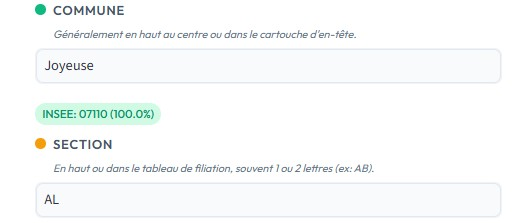
\includegraphics[width=0.65\textwidth]{img/zoom_commune.jpg}
  \caption[Résultat de l'appariement pour le champ Commune]{Résultat de l'appariement : le champ Commune affiche la valeur normalisée \texttt{Joyeuse} avec son code INSEE et un score de confiance de 100\,\%.}
  \label{fig:appariement_commune}
\end{figure}

Ce système automatise la plupart des corrections. Sur les lots testés, plus de 95\,\% des noms de communes erronés sont résolus sans intervention humaine, y compris les cas d'accents manquants, de préfixes abrégés (Saint/St, Sainte/Ste) et de séparateurs variables (tiret, espace, trait d'union).

Dans les départements ruraux et même ailleurs, plusieurs fusions de communes sont intervenues au cours des cinquante dernières années. Par exemple, les anciennes communes de Vallon-Pont-d'Arc et de Lagorce ou les anciennes sections d'Aubenas ont vu leurs dénominations évoluer. Ainsi, lorsqu'un acte ancien mentionne une commune aujourd'hui déléguée ou rattachée, la base de correspondance conserve les anciens codes INSEE associés à leur commune actuelle de rattachement. Le script propose alors à l'opérateur le nom actuel tout en gardant l'ancien nom en note d'archive, afin de garantir la validité du versement sur le portail Géofoncier tout en préservant la valeur du document.

Pour accélérer le calcul lors du traitement de gros volumes de documents, la recherche par correspondance s'appuie sur un index pré-calculé chargé en mémoire au démarrage de l'application. Cet index regroupe les noms de communes par département et par préfixe alphabétique, ce qui réduit le nombre de comparaisons nécessaires et permet d'obtenir une réponse en moins d'une milliseconde par mot.

Pour chaque proposition de correction générée par la comparaison de Levenshtein, l'interface conserve le détail de la chaîne initiale extraite par l'OCR, la méthode de calcul ayant obtenu le meilleur score (directe, par tokens ou partielle), ainsi que les deux communes candidates arrivées en deuxième et troisième positions. Ces informations permettent à l'opérateur de comprendre rapidement l'origine d'une alerte lors d'un doute sur une commune limitrophe.

\subsection{Bilan de la phase de fiabilisation}

La combinaison du nettoyage (correction des erreurs de saisie, résolution des communes, filiation cadastrale) et du contrôle humain via les interfaces web permet d'obtenir des données fiables et directement exploitables. Les incertitudes d'extraction sont rapidement corrigées par l'opérateur, ce qui garantit la qualité finale des bases de données.

Enfin, cette étape de fiabilisation prépare les données pour la dernière phase du projet. Les répertoires propres et les dossiers correctement géolocalisés peuvent à présent être transmis de manière automatique au portail national Géofoncier, sujet présenté dans le chapitre suivant (chapitre~\ref{sec:integration}).





